\documentclass[aspectratio=169,10pt,c]{beamer}

\usepackage[T1]{fontenc}
\usepackage[utf8]{inputenc}
\usepackage{lmodern}
\usepackage{amsmath,amssymb,bm}
\usepackage{booktabs}
\usepackage{graphicx}
\usepackage{tikz}
\usepackage{natbib}
\usepackage{appendixnumberbeamer}
\usetikzlibrary{arrows.meta,positioning,calc}

\graphicspath{{figures/}}
\bibliographystyle{plainnat}

% Scientific palette for path diagrams and data figures only.
\definecolor{fsblue}{HTML}{0072B2}
\definecolor{fsorange}{HTML}{D55E00}
\definecolor{fsgreen}{HTML}{009E73}
\definecolor{fsgray}{HTML}{5F6368}
\definecolor{fsline}{HTML}{DADCE0}

\usetheme{Madrid}
\usecolortheme{beaver}
\setbeamertemplate{navigation symbols}{}
\setbeamertemplate{blocks}[rounded][shadow=false]

\AtBeginDocument{%
  \pdfstringdefDisableCommands{\def\translate#1{#1}}%
}
\newcommand{\wtwo}{W_2}
\newcommand{\Ravg}{\mathcal{R}}
\newcommand{\citefoot}[1]{{\tiny\color{fsgray}\citep{#1}}}
\newcommand{\conceptnote}{{\scriptsize\color{fsgray}Conceptual schematic, not experimental data.}}
\newcommand{\sourcenote}[1]{{\scriptsize\color{fsgray}#1}}

\tikzset{
  box/.style={draw=fsline, rounded corners=1.4pt, align=center,
    font=\scriptsize, inner sep=3.2pt, minimum height=0.72cm},
  arr/.style={-{Latex[length=1.8mm]}, thick, fsblue},
}

\title[Few-step field regularity]{When Averaged Field Regularity Fails to Rank\\ Few-Step Generative Paths}
\author[C.~Callaert]{Cl\'ement Callaert}
\institute[Paris-Saclay]{CentraleSup\'elec and Universit\'e Paris-Saclay}
\date[21 Aug 2026]{PhD interview with Christian Wald \textbullet\ 21 August 2026}

\begin{document}

% -------------------------------------------------------------------------
\begin{frame}
  \titlepage
\end{frame}

% -------------------------------------------------------------------------
\begin{frame}{Generative ODEs and Flow Matching}
  \small
  A continuous normalizing flow is the ODE
  \[
    \frac{dX_t}{dt}=v_\theta(t,X_t),
    \qquad
    X_0\sim p_0,
  \]
  with
  \(
    v_\theta:[0,1]\times\mathbb{R}^d\to\mathbb{R}^d.
  \)
  The input is time and the current state; the output is an instantaneous velocity.

  A generating field \(u_t\) and density \(p_t\) obey the continuity equation
  \[
    \partial_t p_t+\nabla\cdot(p_t u_t)=0.
  \]

  \begin{block}{Flow Matching}
    \[
      \mathcal{L}_{\mathrm{FM}}(\theta)
      =\mathbb{E}_{t,X_t\sim p_t}
      \bigl\|v_\theta(t,X_t)-u_t(X_t)\bigr\|^2.
    \]
  \end{block}

  Once a velocity field is learned, generation requires numerically integrating the ODE.
  \vspace{0.08cm}
  \citefoot{lipman2023flow}
\end{frame}

% -------------------------------------------------------------------------
\begin{frame}{Conditional Flow Matching and stochastic interpolation}
  \footnotesize
  A two-sided interpolant with independent endpoints is
  \[
    X_t=\alpha(t)X_0+\sigma(t)X_1,
    \qquad X_0\perp X_1,
  \]
  with pathwise derivative \(\dot X_t=\dot\alpha(t)X_0+\dot\sigma(t)X_1\).
  The marginal velocity is
  \(
    b_t(x)=\mathbb{E}[\dot X_t\mid X_t=x].
  \)
  This is the same generating field as on the previous slide:
  \(b_t=u_t\).

  \begin{block}{Conditional Flow Matching}
    \[
      \mathcal{L}_{\mathrm{CFM}}(\theta)
      =\mathbb{E}_{t,q(x_1),p_t(x\mid x_1)}
      \bigl\|v_\theta(t,x)-u_t(x\mid x_1)\bigr\|^2.
    \]
    Lipman Theorem~2 then gives
    \(\nabla_\theta\mathcal{L}_{\mathrm{CFM}}=\nabla_\theta\mathcal{L}_{\mathrm{FM}}\).
  \end{block}

  Training uses accessible conditional velocities. Averaging over compatible
  endpoint pairs recovers the marginal field that transports \(p_t\).
  In the Gaussian laboratory below, that field is known exactly:
  \(b(t,x)=A(t)x+c(t)\).
  \vspace{0.06cm}
  \citefoot{lipman2023flow,albergo2025stochastic}
\end{frame}

% -------------------------------------------------------------------------
\begin{frame}{The few-step question}
  \small
  \[
    (\alpha,\sigma)
    \;\longrightarrow\;
    p_t
    \;\longrightarrow\;
    b_t
    \;\longrightarrow\;
    \text{solver stages}
    \;\longrightarrow\;
    \widehat p_1.
  \]
  \textbf{NFE} is the number of evaluations of the velocity field, not the
  number of solver steps. At budget \(B\): Euler uses \(B\) steps, Heun uses
  \(B/2\) steps, RK4 uses \(B/4\) steps.

  Two paths with the same endpoints can induce different fields and different
  errors under the same solver:
  \[
    \text{linear: }(\alpha,\sigma)=(1-t,\,t),
    \qquad
    \text{VP: }\bigl(\cos\tfrac{\pi t}{2},\,\sin\tfrac{\pi t}{2}\bigr).
  \]
  With independent endpoint sampling, the linear interpolant uses the product
  coupling, not an optimal transport coupling.
  Trigonometric VP is not Lipman VP diffusion path (eq.~18).

  \begin{block}{Question}
    Can an averaged regularity score rank probability paths by their
    fixed-NFE endpoint error?
  \end{block}
  \citefoot{lipman2023flow,albergo2025stochastic,liu2023rectified,lipschitzguided2025,sabour2024align}
\end{frame}

% -------------------------------------------------------------------------
\begin{frame}{Exact Gaussian benchmark}
  \footnotesize
  Independent Gaussians \(X_0\sim\mathcal{N}(\mu_0,\Sigma_0)\),
  \(X_1\sim\mathcal{N}(\mu_1,\Sigma_1)\):
  \[
    m_t=\alpha\mu_0+\sigma\mu_1,
    \quad
    Q(t)=\alpha^2\Sigma_0+\sigma^2\Sigma_1,
    \quad
    C_t=\dot\alpha\,\alpha\,\Sigma_0+\dot\sigma\,\sigma\,\Sigma_1.
  \]
  \[
    b(t,x)=A(t)x+c(t),
    \qquad
    A(t)=C_t Q(t)^{-1},
    \qquad
    c(t)=\dot m_t-A(t)m_t,
  \]
  with \(A(t)\in\mathbb{R}^{d\times d}\) and \(c(t),x,b(t,x)\in\mathbb{R}^d\).

  \begin{columns}[T,onlytextwidth]
    \begin{column}{0.46\textwidth}
      \begin{center}
      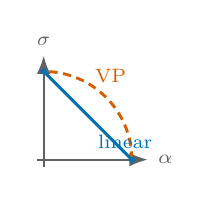
\begin{tikzpicture}[scale=1.12, thick]
        \draw[-{Latex}, fsgray] (-0.08,0) -- (1.18,0) node[right,font=\scriptsize] {$\alpha$};
        \draw[-{Latex}, fsgray] (0,-0.08) -- (0,1.18) node[above,font=\scriptsize] {$\sigma$};
        \draw[fsblue, line width=1.05pt] (1,0) -- (0,1);
        \draw[fsorange, line width=1.05pt, densely dashed]
          (1,0) arc (0:90:1);
        \fill[fsblue] (1,0) circle (1.0pt);
        \fill[fsblue] (0,1) circle (1.0pt);
        \node[font=\scriptsize, fsblue, anchor=west] at (0.50,0.20) {linear};
        \node[font=\scriptsize, fsorange, anchor=south] at (0.76,0.76) {VP};
      \end{tikzpicture}
      \end{center}
      \sourcenote{Coefficient plane (schematic).}
    \end{column}
    \begin{column}{0.52\textwidth}
      A controlled Gaussian laboratory isolates discretization error:
      \begin{itemize}\itemsep=0.12em
        \item exact marginal field
        \item no neural-network training error
        \item numerical endpoint remains Gaussian
        \item Gaussian \(\wtwo\) is available in closed form
        \item solver discretization is isolated
      \end{itemize}
    \end{column}
  \end{columns}
  \vspace{0.04cm}
  \citefoot{albergo2025stochastic,lipman2023flow,gelbrich1990formula}
\end{frame}

% -------------------------------------------------------------------------
\begin{frame}{Candidate regularity criterion}
  \small
  Chen, Vanden-Eijnden, and Xu use averaged squared Jacobian Lipschitzness.
  For the affine field, \(\nabla_x b(t,x)=A(t)\) is state-independent, so
  \[
    \Ravg[b]
    =\int_0^1 \mathbb{E}\bigl[\|\nabla_x b(t,X_t)\|_2^2\bigr]\,dt
    =\int_0^1 \|A(t)\|_2^2\,dt.
  \]
  Here \(\|\cdot\|_2\) is the spectral operator 2-norm, as implemented.

  This quantity is a plausible stability or error-control proxy. Controlling
  or upper-bounding an error is weaker than correctly ordering two paths at
  a fixed small NFE. \(\Ravg\) averages over \([0,1]\); a solver samples
  finitely many stages.

  \vspace{0.06cm}
  \begin{center}
  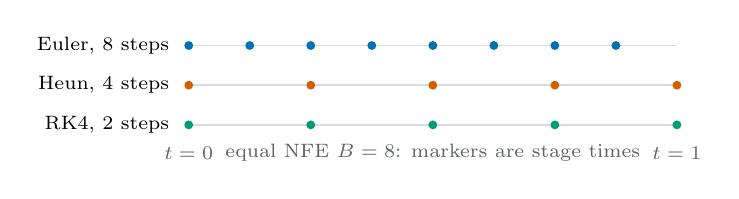
\begin{tikzpicture}[x=6.2cm, y=0.42cm, font=\scriptsize]
    \node[anchor=east] at (-0.02,2.4) {Euler, 8 steps};
    \draw[fsline, line width=0.7pt] (0,2.4) -- (1,2.4);
    \foreach \t in {0,0.125,0.25,0.375,0.5,0.625,0.75,0.875} {
      \fill[fsblue] (\t,2.4) circle (1.6pt);
    }
    \node[anchor=east] at (-0.02,1.2) {Heun, 4 steps};
    \draw[fsline, line width=0.7pt] (0,1.2) -- (1,1.2);
    \foreach \t in {0,0.25,0.5,0.75,1} {
      \fill[fsorange] (\t,1.2) circle (1.6pt);
    }
    \node[anchor=east] at (-0.02,0.0) {RK4, 2 steps};
    \draw[fsline, line width=0.7pt] (0,0.0) -- (1,0.0);
    \foreach \t in {0,0.25,0.5,0.75,1} {
      \fill[fsgreen] (\t,0.0) circle (1.6pt);
    }
    \node[font=\scriptsize, fsgray] at (0,-0.85) {$t=0$};
    \node[font=\scriptsize, fsgray] at (1,-0.85) {$t=1$};
    \node[font=\scriptsize, fsgray] at (0.5,-0.85) {equal NFE $B=8$: markers are stage times};
  \end{tikzpicture}
  \end{center}
  \citefoot{lipschitzguided2025}
\end{frame}

% -------------------------------------------------------------------------
\begin{frame}{Frozen experimental protocol}
  \small
  Each comparison holds target, solver, and NFE fixed, then compares linear
  versus VP. Source \(N(0,I)\). Equal-NFE accounting throughout.

  \vspace{0.12cm}
  \begin{center}
  \begin{tabular}{ll}
    \toprule
    factor & frozen grid \\
    \midrule
    targets & anisotropic (condition 4), seeded low-rank \\
    dimensions & \(d\in\{2,8\}\) \\
    paths & linear vs trigonometric VP \\
    solvers & Euler, Heun, RK4 \\
    NFE & \(8\), \(16\), \(32\) \\
    configurations & \(72\) \\
    paired comparisons & \(36\) \\
    endpoint metric & Gelbrich \(\wtwo\) \\
    precision & 80-digit audit of all \(72\) values \\
    \bottomrule
  \end{tabular}
  \end{center}

  \vspace{0.18cm}
  14 ranking inversions among 36 prespecified paired comparisons in the
  frozen grid.
  \vspace{0.08cm}
  \sourcenote{Data: \texttt{phase4\_gaussian\_reproduction\_2026-07-24-v1:results}.}
\end{frame}

% -------------------------------------------------------------------------
\begin{frame}{Main result}
  \begin{center}
  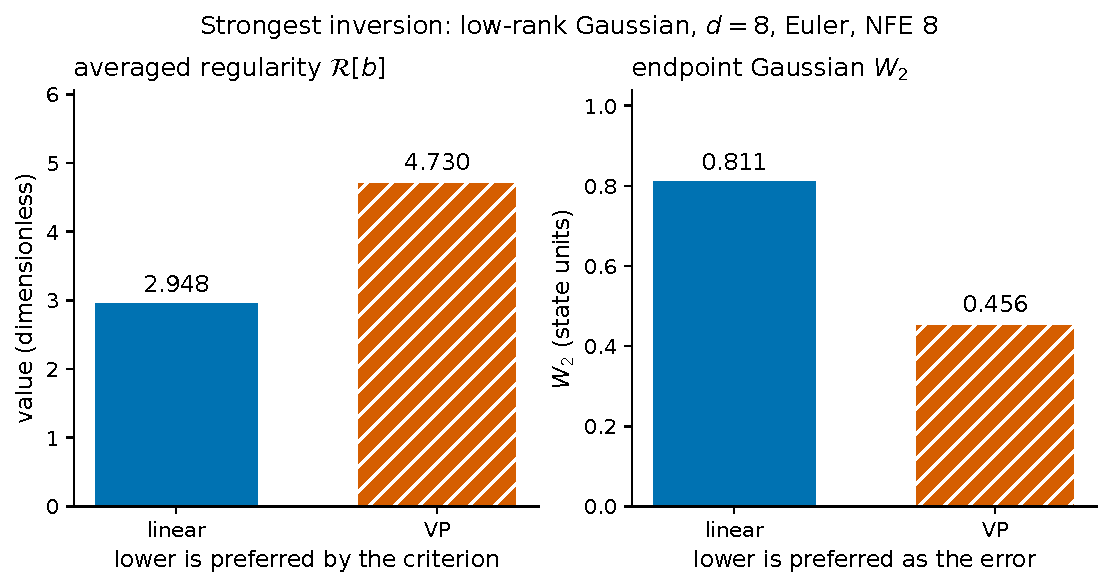
\includegraphics[width=0.92\textwidth,height=0.44\textheight,keepaspectratio]{fig_strongest_inversion.pdf}
  \end{center}
  \sourcenote{Experimental data. Strongest inversion: low-rank Gaussian,
  \(d=8\), Euler, NFE 8, metric \(\wtwo\).
  Linear \(\Ravg=2.9476523251\), \(\wtwo=0.8108540111\);
  VP \(\Ravg=4.7295206355\), \(\wtwo=0.4564779075\);
  margin \(0.3543761036\) (linear \(\wtwo\) is 78\% larger).
  Lower is preferred on both axes.}

  \vspace{0.08cm}
  \begin{block}{Result}
    In this controlled commuting Gaussian benchmark, lower averaged
    regularity does not necessarily imply lower fixed-NFE endpoint error.
  \end{block}
\end{frame}

% -------------------------------------------------------------------------
\begin{frame}{Mechanism: signed and transported defects}
  \footnotesize
  Centered commuting mode \(x_i'=a_i(t)x_i\). Exact one-step factor
  \(e_{i,n}=\sqrt{q_i(t_{n+1})/q_i(t_n)}\). A Runge-Kutta step multiplies by
  \(r_{i,n}\). With \(S\) steps,
  \[
    \prod_{n<S} r_{i,n}-\prod_{n<S} e_{i,n}
    =\sum_{n<S}(r_{i,n}-e_{i,n})
    \Bigl(\prod_{j<n}r_{i,j}\Bigr)
    \Bigl(\prod_{j>n}e_{i,j}\Bigr).
  \]
  Earlier factors are numerical, later factors are exact. No smallness
  assumption. Each local defect \(r_{i,n}-e_{i,n}\) is signed; later dynamics
  transport it; defects can cancel; endpoint error depends on stage locations.
  An unsigned time average of \(\|A\|_2^2\) does not encode those cancellations.

  \vspace{0.06cm}
  \begin{center}
  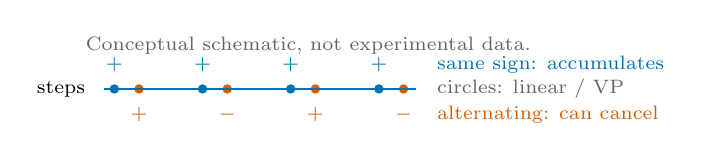
\begin{tikzpicture}[font=\scriptsize, x=1.12cm, y=0.48cm]
    \node[font=\scriptsize\color{fsgray}] at (2.2, 2.25) {\conceptnote};
    \foreach \x in {0,1,2,3} {
      \fill[fsblue] (\x,1.10) circle (1.7pt);
      \fill[fsorange] (\x+0.28,1.10) circle (1.7pt);
    }
    \draw[fsblue, line width=1.0pt] (-0.12,1.10) -- (3.42,1.10);
    \node[anchor=east] at (-0.22,1.10) {steps};
    \node[fsblue] at (0.0,1.75) {$+$};
    \node[fsblue] at (1.0,1.75) {$+$};
    \node[fsblue] at (2.0,1.75) {$+$};
    \node[fsblue] at (3.0,1.75) {$+$};
    \node[fsorange] at (0.28,0.42) {$+$};
    \node[fsorange] at (1.28,0.42) {$-$};
    \node[fsorange] at (2.28,0.42) {$+$};
    \node[fsorange] at (3.28,0.42) {$-$};
    \node[anchor=west, fsblue] at (3.55,1.75) {same sign: accumulates};
    \node[anchor=west, fsorange] at (3.55,0.42) {alternating: can cancel};
    \node[anchor=west, font=\scriptsize, fsgray] at (3.55,1.10) {circles: linear / VP};
  \end{tikzpicture}
  \end{center}
\end{frame}

% -------------------------------------------------------------------------
\begin{frame}{Grid-aware Euler construction}
  \footnotesize
  Fix \(L>0\) and integer \(N\ge 1\), \(h=1/N\), left-endpoint Euler nodes
  \(t_n=n/N\). Set \(\epsilon_N=N(e^{L/N}-1)-L>0\) and
  \(a_0(t)=L\), \(a_{1,N}(t)=L+\epsilon_N\cos(2\pi Nt)\).

  \begin{columns}[T,onlytextwidth]
    \begin{column}{0.58\textwidth}
      \[
        \int_0^1 a_0=\int_0^1 a_{1,N}=L,
        \qquad
        \text{exact endpoints }e^{L}.
      \]
      \[
        \int_0^1 a_{1,N}^2
        =L^2+\tfrac12\epsilon_N^2
        >L^2=\int_0^1 a_0^2.
      \]
      At every node, \(\cos(2\pi Nt_n)=1\), so
      \(1+a_{1,N}(t_n)/N=e^{L/N}\) and
      \(\prod_{n=0}^{N-1}(1+a_{1,N}(t_n)/N)=e^{L}\).
      For the constant field, \((1+L/N)^N<e^{L}\).
    \end{column}
    \begin{column}{0.40\textwidth}
      \begin{center}
      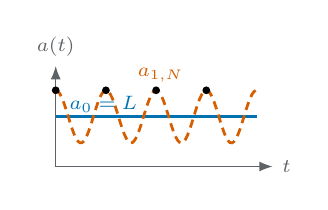
\begin{tikzpicture}[x=2.55cm, y=0.88cm, font=\scriptsize]
        \draw[-{Latex}, fsgray] (0,0.50) -- (1.08,0.50) node[right] {$t$};
        \draw[-{Latex}, fsgray] (0,0.50) -- (0,1.95) node[above] {$a(t)$};
        \draw[fsblue, line width=1.0pt] (0,1.22) -- (1,1.22);
        \draw[fsorange, line width=1.0pt, densely dashed]
          plot[domain=0:1, samples=100]
          (\x, {1.22 + 0.38*cos(360*4*\x)});
        \foreach \k in {0,1,2,3} {
          \fill[black] ({0.25*\k}, {1.22+0.38}) circle (1.4pt);
        }
        \node[fsblue, font=\scriptsize, anchor=west] at (0.02,1.40) {$a_0=L$};
        \node[fsorange, font=\scriptsize, anchor=west] at (0.36,1.82) {$a_{1,N}$};
      \end{tikzpicture}
      \end{center}
      \sourcenote{Schematic, \(N=4\) shown. Not experimental data.}
    \end{column}
  \end{columns}

  On this frozen grid, the higher-regularity field is integrated exactly,
  while the lower-regularity constant field is not.
  The field \(a_{1,N}\) is chosen after the grid \(N\).
\end{frame}

% -------------------------------------------------------------------------
\begin{frame}{Scope and limitations}
  \footnotesize
  \begin{columns}[T,onlytextwidth]
    \begin{column}{0.48\textwidth}
      {\color{fsblue}\textbf{What the study establishes}}
      \begin{itemize}\itemsep=0.14em
        \item exact affine Gaussian benchmark
        \item frozen-grid empirical inversions
        \item signed transported-defect identity
        \item explicit grid-aware Euler non-implication
      \end{itemize}
    \end{column}
    \begin{column}{0.50\textwidth}
      {\color{fsorange}\textbf{Current limitations}}
      \begin{itemize}\itemsep=0.10em
        \item commuting Gaussian covariances
        \item affine exact fields, not learned fields
        \item two main path families
        \item a finite solver and NFE grid
        \item Euler construction is grid-aware
        \item identity-style ODE parameterization
        \item exponential integrators are exact here
        \item no direct theorem for CTMC samplers
      \end{itemize}
    \end{column}
  \end{columns}

  \vspace{0.16cm}
  Next experiments: non-commuting covariances, learned fields, adaptive or
  optimized schedules, non-affine systems, and discrete rate-based samplers.
  \vspace{0.06cm}
  \citefoot{lu2022dpmsolver,zhang2023deis}
\end{frame}

% -------------------------------------------------------------------------
\begin{frame}{Conclusion}
  \small
  \begin{enumerate}\itemsep=0.35em
    \item Averaged field regularity may be useful for control or bounds, but
          it is insufficient by itself to rank fixed-NFE sampling paths in
          the tested benchmark.
    \item Few-step endpoint error is governed by signed local defects, solver
          stage locations, propagation, and cancellation.
    \item The controlled Gaussian model provides an exact diagnostic
          environment and an explicit non-implication example.
  \end{enumerate}

  \vspace{0.18cm}
  \begin{block}{Research direction}
    For discrete generative models, the analogous question is how a
    probability path, its time-dependent rates, and a finite-step CTMC
    solver interact under a fixed computational budget.
  \end{block}
\end{frame}

% =========================================================================
\appendix
\section{Technical appendix}

\begin{frame}{A1. Equal-NFE accounting}
  \small
  NFE counts \texttt{evaluate} calls. Bookkeeping is not NFE.
  \[
    n_{\mathrm{steps}} = B\big/\text{evals per step},
    \qquad B \bmod \text{evals per step} = 0.
  \]
  \begin{center}
  \begin{tabular}{lccc}
    \toprule
    solver & evals / step & steps at \(B=8\) & steps at \(B=32\) \\
    \midrule
    Euler & 1 & 8 & 32 \\
    Heun  & 2 & 4 & 16 \\
    RK4   & 4 & 2 & 8 \\
    \bottomrule
  \end{tabular}
  \end{center}
  \vspace{0.18cm}
  A higher-order solver receives fewer, more informative steps at the same
  field-evaluation budget. Equal step count would not be an equal-compute
  comparison.
\end{frame}

\begin{frame}{A2. Affine Gaussian field}
  \small
  \(X_0\sim\mathcal{N}(\mu_0,\Sigma_0)\), \(X_1\sim\mathcal{N}(\mu_1,\Sigma_1)\)
  independent in \(\mathbb{R}^d\). Interpolant \(X_t=\alpha X_0+\sigma X_1\).
  Joint-Gaussian conditioning gives
  \[
    b_t(x)=\dot m_t+C_t Q(t)^{-1}(x-m_t),
  \]
  hence \(A(t)=C_t Q(t)^{-1}\) and \(c(t)=\dot m_t-A(t)m_t\).
  Then \(b(t,\cdot):\mathbb{R}^d\to\mathbb{R}^d\), \(A(t)\in\mathbb{R}^{d\times d}\),
  \(c(t)\in\mathbb{R}^d\). Centered with \(\Sigma_0=I\):
  \(A=\tfrac12 Q'Q^{-1}\), \(c=0\).
  This is the stochastic-interpolant marginal ODE.
  Linear \((1-t,t)\) is independent coupling. It is not automatically a global
  OT coupling.
  \citefoot{albergo2025stochastic,gelbrich1990formula}
\end{frame}

\begin{frame}{A3. Gelbrich \texorpdfstring{$\wtwo$}{W2} and \texorpdfstring{$|r_i|$}{|r i|}}
  \small
  For Gaussians,
  \[
    \wtwo^2
    =\|\hat m-\mu_1\|_2^2
    +\mathrm{tr}\Bigl(\hat C+\Sigma_1
    -2\bigl(\Sigma_1^{1/2}\hat C\Sigma_1^{1/2}\bigr)^{1/2}\Bigr).
  \]
  Reported values are \(\wtwo=\sqrt{\wtwo^2}\), not \(\wtwo^2\).
  In the centered commuting case, with numerical modal factors \(r_i\),
  \[
    \wtwo^2=\sum_{i=1}^d \bigl(|r_i|-\sqrt{\lambda_i}\bigr)^2.
  \]
  The absolute value is required if a coarse Euler factor is negative.
  \citefoot{gelbrich1990formula}
\end{frame}

\begin{frame}{A4. Local defects, exact minus method}
  \small
  For \(x'=a(t)x\) with smooth \(a\), the leading coefficients of the local
  defect (exact factor minus method factor) are
  \[
    \delta_{\mathrm{Euler}}=\tfrac12(a'+a^2)h^2+O(h^3),
    \qquad
    \delta_{\mathrm{Heun}}=\bigl(-\tfrac1{12}a''+\tfrac16 a^3\bigr)h^3+O(h^4).
  \]
  Euler and Heun sample different derivatives and different stages.
  RK4 is compared through its exact scalar stage polynomial against
  \(\sqrt{q_i(t_{n+1})/q_i(t_n)}\). No memorized non-autonomous RK4 leading
  formula is used.
\end{frame}

\begin{frame}{A5. Numerical precision}
  \small
  All 72 float64 \(\wtwo\) values versus an 80-digit reference:
  \begin{itemize}
    \item maximum absolute difference \(9.7050430488\times 10^{-10}\)
    \item smallest inversion margin \(1.1188920612\times 10^{-5}\)
    \item ratio greater than \(11{,}500\)
  \end{itemize}
  Source: \texttt{phase4\_precision\_2026-07-24-v1}.
  Mixture evidence was excluded after estimator calibration failure.
\end{frame}

\begin{frame}{A6. All 14 inversion margins}
  \begin{center}
  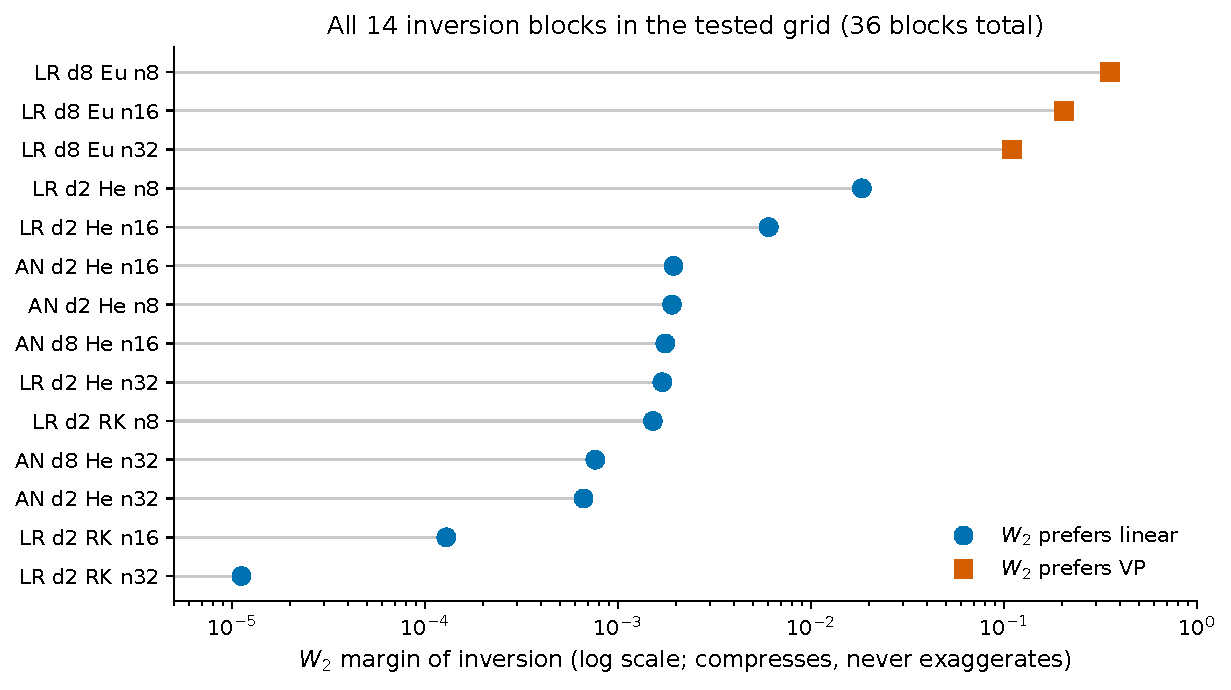
\includegraphics[width=0.92\textwidth,height=0.62\textheight,keepaspectratio]{fig_inversions14.pdf}
  \end{center}
  \sourcenote{Experimental data. Frozen Phase~4 grid. Logarithmic axis
  compresses, never exaggerates, magnitudes.}
\end{frame}

\begin{frame}{A7. Non-centered replication}
  \small
  Pre-registered family: source \(\mathcal{N}(\mu_0,I)\) with
  \(\mu_{0,i}=0.75(-1)^i\), target \(\mathcal{N}(\mu_1,D)\) with geometric
  spectrum of condition number 6, so \(c(t)\neq 0\).
  \begin{itemize}
    \item 11 of 18 blocks invert
    \item \(\Ravg\) prefers VP (margin \(0.7513\)) because \(\Ravg\) ignores \(c(t)\) by definition
    \item \(\wtwo\) prefers linear in those inverted blocks
    \item all 11 pass the 80-digit audit
  \end{itemize}
  Still Gaussian, diagonal, and commuting. Supporting replication, not
  out-of-distribution evidence.
\end{frame}

\begin{frame}{A8. Solver-path interaction}
  \begin{center}
  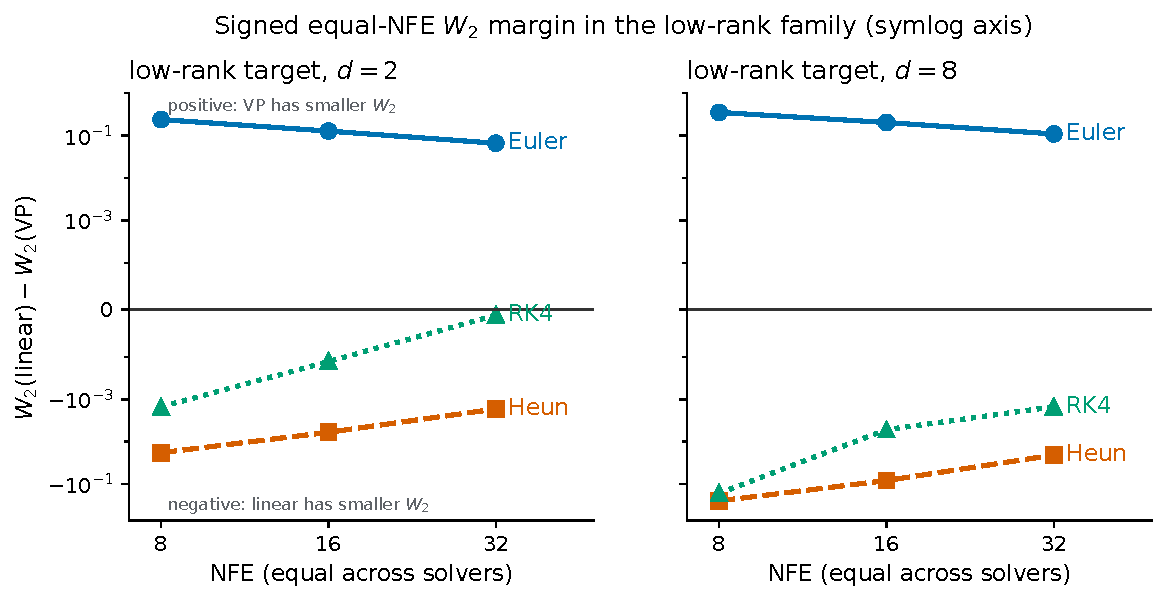
\includegraphics[width=0.95\textwidth,height=0.58\textheight,keepaspectratio]{fig_interaction.pdf}
  \end{center}
  \sourcenote{Experimental data. Positive: VP has smaller \(\wtwo\).
  Negative: linear has smaller \(\wtwo\). Low-rank family only. Equal NFE.
  Source: frozen Phase~4 results.}
\end{frame}

\begin{frame}{A9. Strongest-block modal split}
  \begin{center}
  
\includegraphics[width=0.95\textwidth,height=0.56\textheight,keepaspectratio]{fig_eigenmode.pdf}
  \end{center}
  \sourcenote{Experimental data. Uses \(\wtwo^2\) modal contributions, not
  \(\wtwo\). Decomposition table is post-hoc relative to the Phase~3 gate.
  Dominant mode (index 7) accounts for the bulk of the linear error.}
\end{frame}

\begin{frame}{A10. Averaged regularity proposal}
  \small
  Definition 3.2 of Chen, Vanden-Eijnden, and Xu is
  \(A_2=\int_0^1 \mathbb{E}[\|\nabla b_t(I_t)\|_2^2]\,dt\), spectral 2-norm.
  The paper also gives a transfer formula that optimizes a schedule
  relative to a linear reference, typically under a constraint such as
  \(\alpha^2+\sigma^2=1\).
  This talk ranks two fixed paths at the identity time parameterization.
  Reparameterization-based schedule optimization is a complementary use that
  the result does not address.
  \citefoot{lipschitzguided2025}
\end{frame}

\begin{frame}{A11. Exponential integrators}
  \small
  DPM-Solver, DPM-Solver++, and DEIS integrate a linear component exactly
  and approximate the remainder.
  On the present affine Gaussian fields those methods are exact, so the
  ranking question is vacuous for them.
  Learned fields are not affine. The limitation study therefore concerns
  generic fixed-stage Runge-Kutta discretization, which remains relevant
  when the field is nonlinear.
  \citefoot{lu2022dpmsolver,lu2022dpmsolverpp,zhang2023deis}
\end{frame}

\begin{frame}{A12. CTMC analogy}
  \small
  In a continuous-time Markov chain the generator \(Q_t(x,y)\) plays the role
  of \(b_t(x)\): it is the dynamical object that is discretized.
  A few-step rate model likewise chooses a path (or rate schedule), an
  approximation scheme, and a budget.
  The analogue of NFE is the number of generator or rate evaluations,
  or the number of accepted jumps, depending on the scheme.
  Nothing in the Gaussian ODE study proves a statement about CTMCs.
  The transferable discipline is: isolate a reduced ranking statistic,
  then test whether it actually orders endpoint error at fixed budget.
\end{frame}

\begin{frame}[allowframebreaks]{A13. References}
  \tiny
  \bibliography{references}
\end{frame}

\end{document}
